%\PassOptionsToPackage{table}{xcolor}
% \documentclass[smaller, dvipsnames,handout,
% hyperref={colorlinks=true,urlcolor=magenta,citecolor=cyan,linkcolor=orange}]{beamer}
\def\bmode{0} % Mode 0 for presentation, mode 1 for a handout with notes, mode 2 fo% r handout without notes
\if 0\bmode
\documentclass[usenames,dvipsnames,smaller]{beamer}
\else \if 1\bmode
\immediate\write18{pdflatex -jobname=\jobname-Handout-Notes\space\jobname}
\documentclass[usenames,dvipsnames,smaller,handout]{beamer}
\usepackage{handoutWithNotes}
\pgfpagesuselayout{2 on 1 with notes}[letterpaper, landscape, border shrink=4mm]
\else \if 2\bmode
\immediate\write18{pdflatex -jobname=\jobname-Handout\space\jobname}
\documentclass[usenames,dvipsnames,smaller,handout]{beamer}
\fi
\fi
\fi


% \documentclass[smaller,handout
% ]{beamer}
%\usepackage{etex}
%\newcommand{\num}{6{} }

% \usetheme[
%   outer/progressbar=foot,
%   outer/numbering=counter,
%  block=fill
% ]{metropolis}

%\useoutertheme{metropolis}

\usetheme{Madrid}
\useoutertheme[subsection=false]{miniframes} % Alternatively: miniframes, infolines, split
\useinnertheme{circles}
\usecolortheme{seahorse}

\usepackage[backend=biber,style=authoryear,maxcitenames=2,maxbibnames=99,safeinputenc,url=false,
eprint=false]{biblatex}
\addbibresource{bib/references.bib}
\AtEveryCitekey{\iffootnote{{\tiny}\tiny}{\tiny}}

%\usepackage{pgfpages}
%\setbeameroption{hide notes} % Only slides
%\setbeameroption{show only notes} % Only notes
%\setbeameroption{hide notes} % Only notes
%\setbeameroption{show notes on second screen=right} % Both

% \usepackage[sfdefault]{Fira Sans}

% \setsansfont[BoldFont={Fira Sans}]{Fira Sans Light}
% \setmonofont{Fira Mono}

%\usepackage{fira}
%\setsansfont{Fira}
%\setmonofont{Fira Mono}
% To give a presentation with the Skim reader (http://skim-app.sourceforge.net) on OSX so
% that you see the notes on your laptop and the slides on the projector, do the following:
% 
% 1. Generate just the presentation (hide notes) and save to slides.pdf
% 2. Generate onlt the notes (show only nodes) and save to notes.pdf
% 3. With Skim open both slides.pdf and notes.pdf
% 4. Click on slides.pdf to bring it to front.
% 5. In Skim, under "View -> Presentation Option -> Synhcronized Noted Document"
%    select notes.pdf.
% 6. Now as you move around in slides.pdf the notes.pdf file will follow you.
% 7. Arrange windows so that notes.pdf is in full screen mode on your laptop
%    and slides.pdf is in presentation mode on the projector.

% Give a slight yellow tint to the notes page
%\setbeamertemplate{note page}{\pagecolor{yellow!5}\insertnote}\usepackage{palatino}


%\usetheme{metropolis}
%\usecolortheme{beaver}
%\usepackage{xcolor}
\definecolor{darkcandyapplered}{HTML}{A40000}
\definecolor{lightcandyapplered}{HTML}{e74c3c}

%\setbeamercolor{title}{fg=darkcandyapplered}
%\setbeamercolor{frametitle}{bg=darkcandyapplered!80!black!90!white}
%\setbeamertemplate{frametitle}{\bf\insertframetitle}
%\setbeamercolor{footnote mark}{fg=darkcandyapplered}
%\setbeamercolor{footnote}{fg=darkcandyapplered!70}
%\Raggedbottom
%\setbeamerfont{page number in head/foot}{size=\tiny}
%\usepackage[tracking]{microtype}


\setbeamertemplate{frametitle}{%
    \nointerlineskip%
    \begin{beamercolorbox}[wd=\paperwidth,ht=2.0ex,dp=0.6ex]{frametitle}
        \hspace*{1ex}\insertframetitle%
    \end{beamercolorbox}%
}



\setbeamerfont{caption}{size=\footnotesize}
\setbeamercolor{caption name}{fg=darkcandyapplered}


%\usepackage[sc,osf]{mathpazo}   % With old-style figures and real smallcaps.
%\linespread{1.025}              % Palatino leads a little more leading

% Euler for math and numbers
%\usepackage[euler-digits,small]{eulervm}
%\AtBeginDocument{\renewcommand{\hbar}{\hslash}}
\usepackage{graphicx,multirow,paralist,booktabs}


%\mode<presentation> { \setbeamercovered{transparent} }

\setbeamertemplate{navigation symbols}{}
\makeatletter
\def\beamerorig@set@color{%
  \pdfliteral{\current@color}%
  \aftergroup\reset@color
}
\def\beamerorig@reset@color{\pdfliteral{\current@color}}
\makeatother

%=== GRAPHICS PATH ===========
\graphicspath{{./m3-images/}}
% Marginpar width
%Marginpar width
%\setlength{\marginparsep}{.02in}


%% Captions
% \usepackage{caption}
% \captionsetup{
%   labelsep=quad,
%   justification=raggedright,
%   labelfont=sc
% }

%AMS-TeX packages

\usepackage{amssymb,amsmath,amsthm} 
\usepackage{bm}
\usepackage{color}

\usepackage{hyperref,enumerate}
\usepackage{minitoc,array}


%https://tex.stackexchange.com/a/31370/2269
\usepackage{mathtools,cancel}

\renewcommand{\CancelColor}{\color{red}} %change cancel color to red

\makeatletter
\let\my@cancelto\cancelto %copy over the original cancelto command
\newcommand<>{\cancelto}[2]{\alt#3{\my@cancelto{#1}{#2}}{\mathrlap{#2}\phantom{\my@cancelto{#1}{#2}}}}
% redefine the cancelto command, using \phantom to assure that the
% result doesn't wiggle up and down with and without the arrow
\makeatother


\definecolor{slblue}{rgb}{0,.3,.62}
\hypersetup{
    colorlinks,%
    citecolor=blue,%
    filecolor=blue,%
    linkcolor=blue,
    urlcolor=slblue
}

%%% TIKZ
\usepackage{animate}
\usepackage{tikz}
\usepackage{pgfplots}
\usepackage{pgfplotstable}
\usepackage{pgfgantt}
\usepackage{tikzsymbols}
\pgfplotsset{compat=newest}
\usepgfplotslibrary{groupplots,fillbetween}

\usetikzlibrary{arrows,shapes,positioning,shapes.geometric}
\usetikzlibrary{decorations.markings}
\usetikzlibrary{shadows,automata}
\usetikzlibrary{patterns,matrix}
\usetikzlibrary{trees,mindmap,backgrounds}
%\usetikzlibrary{circuits.ee.IEC}
\usetikzlibrary{decorations.text}
% For Sagnac Picture
\usetikzlibrary{%
    decorations.pathreplacing,%
    decorations.pathmorphing%
}
\tikzset{no shadows/.style={general shadow/.style=}}
%
%\usepackage{paralist}



%%% FORMAT PYTHON CODE
%\usepackage{listings}
% Default fixed font does not support bold face
\DeclareFixedFont{\ttb}{T1}{txtt}{bx}{n}{8} % for bold
\DeclareFixedFont{\ttm}{T1}{txtt}{m}{n}{8}  % for normal

% Custom colors
\definecolor{deepblue}{rgb}{0,0,0.5}
\definecolor{deepred}{rgb}{0.6,0,0}
\definecolor{deepgreen}{rgb}{0,0.5,0}

%\usepackage{listings}

% Python style for highlighting
% \newcommand\pythonstyle{\lstset{
% language=Python,
% basicstyle=\footnotesize\ttm,
% otherkeywords={self},             % Add keywords here
% keywordstyle=\footnotesize\ttb\color{deepblue},
% emph={MyClass,__init__},          % Custom highlighting
% emphstyle=\footnotesize\ttb\color{deepred},    % Custom highlighting style
% stringstyle=\color{deepgreen},
% frame=tb,                         % Any extra options here
    % showstringspaces=false            % 
% }}

% % Python environment
% \lstnewenvironment{python}[1][]
% {
% \pythonstyle
% \lstset{#1}
% }
% {}

% % Python for external files
% \newcommand\pythonexternal[2][]{{
% \pythonstyle
% \lstinputlisting[#1]{#2}}}

% Python for inline
% 
% \newcommand\pythoninline[1]{{\pythonstyle\lstinline!#1!}}


\newcommand{\osn}{\oldstylenums}
\newcommand{\dg}{^{\circ}}
\newcommand{\lt}{\left}
\newcommand{\rt}{\right}
\newcommand{\pt}{\phantom}
\newcommand{\tf}{\therefore}
\newcommand{\?}{\stackrel{?}{=}}
\newcommand{\fr}{\frac}
\newcommand{\dfr}{\dfrac}
\newcommand{\ul}{\underline}
\newcommand{\tn}{\tabularnewline}
\newcommand{\nl}{\newline}
\newcommand\relph[1]{\mathrel{\phantom{#1}}}
\newcommand{\cm}{\checkmark}
\newcommand{\ol}{\overline}
\newcommand{\rd}{\color{red}}
\newcommand{\bl}{\color{blue}}
\newcommand{\pl}{\color{purple}}
\newcommand{\og}{\color{orange!90!black}}
\newcommand{\gr}{\color{green!40!black}}
\newcommand{\nin}{\noindent}
\newcommand{\la}{\lambda}
\renewcommand{\th}{\theta}
\newcommand{\al}{\alpha}
\newcommand{\G}{\Gamma}
\newcommand*\circled[1]{\tikz[baseline=(char.base)]{
            \node[shape=circle,draw,thick,inner sep=1pt] (char) {\small #1};}}

\newcommand{\bc}{\begin{compactenum}[\quad--]}
\newcommand{\ec}{\end{compactenum}}

\newcommand{\p}{\partial}
\newcommand{\pd}[2]{\frac{\partial{#1}}{\partial{#2}}}
\newcommand{\dpd}[2]{\dfrac{\partial{#1}}{\partial{#2}}}
\newcommand{\pdd}[2]{\frac{\partial^2{#1}}{\partial{#2}^2}}


\pgfmathdeclarefunction{poiss}{1}{%
  \pgfmathparse{(#1^x)*exp(-#1)/(x!)}%
  }

\pgfmathdeclarefunction{gauss}{2}{%
  \pgfmathparse{1/(#2*sqrt(2*pi))*exp(-((x-#1)^2)/(2*#2^2))}%
}

\pgfmathdeclarefunction{expo}{2}{%
  \pgfmathparse{#1*exp(-#1*#2)}%
}

\pgfmathdeclarefunction{expocdf}{2}{%
  \pgfmathparse{1 -exp(-#1*#2)}%
}

\makeatletter
\long\def\ifnodedefined#1#2#3{%
    \@ifundefined{pgf@sh@ns@#1}{#3}{#2}%
}

\pgfplotsset{
    discontinuous/.style={
    scatter,
    scatter/@pre marker code/.code={
        \ifnodedefined{marker}{
            \pgfpointdiff{\pgfpointanchor{marker}{center}}%
             {\pgfpoint{0}{0}}%
             \ifdim\pgf@y>0pt
                \tikzset{options/.style={mark=*, fill=white}}
                \draw [densely dashed] (marker-|0,0) -- (0,0);
                \draw plot [mark=*] coordinates {(marker-|0,0)};
             \else
                \tikzset{options/.style={mark=none}}
             \fi
        }{
            \tikzset{options/.style={mark=none}}        
        }
        \coordinate (marker) at (0,0);
        \begin{scope}[options]
    },
    scatter/@post marker code/.code={\end{scope}}
    }
}

\makeatother

%%%%%%%%%%%%%%%%%%%%%%%%%%%%%%%%%%%%%%%%%%%%%%%%%%%
%%%%%%%%%%%%%%%%%%%%%%%%%%%%%%%%%%%%%%%%%%%%%%%%%%%

\title[CEE 260/MIE 273 M3c: Lognormal \& Exponential]{{\normalsize CEE 260/MIE 273: Probability and Statistics in Civil Engineering} \\
Lecture M3c: Lognormal and Exponential Distributions}
\date[\today]{\footnotesize \today}
\author{{\bf Jimi Oke}}
\institute[UMass Amherst]{
  \begin{tikzpicture}[baseline=(current bounding box.center)]
    \node[anchor=base] at (-7,0) (its) {
\includegraphics[scale=.3]{UMassEngineering_vert}} ;
  \end{tikzpicture}
}



%https://tex.stackexchange.com/questions/55806/mindmap-tikzpicture-in-beamer-reveal-step-by-step
  \tikzset{
    invisible/.style={opacity=0},
    visible on/.style={alt={#1{}{invisible}}},
    alt/.code args={<#1>#2#3}{%
      \alt<#1>{\pgfkeysalso{#2}}{\pgfkeysalso{#3}} % \pgfkeysalso doesn't change the path
    },
  }


\usepackage{listings}

\lstset{language=matlab,
                basicstyle=\scriptsize\ttfamily,
                keywordstyle=\color{blue}\ttfamily,
                stringstyle=\color{blue}\ttfamily,
                commentstyle=\color{gray}\ttfamily,
                morecomment=[l][\color{gray}]{\#}
              }
         
\begin{document}

\maketitle




\begin{frame}
  \frametitle{Outline}
  \tableofcontents
\end{frame}



 
\section{Introduction}
\begin{frame}
  \frametitle{Recap of normal distribution}
  \pause

  \begin{itemize}
  \item The {\gr PDF} of the normal distribution (parameters $\mu$ and $\sigma^{2}$) is given by \pause
    \begin{equation}\gr
      f_{X}(x) = \fr{1}{\sigma\sqrt{2\pi}}\exp\lt[\fr{1}{2}\lt(\fr{x - \mu}{\sigma}\rt)^{2}\rt]
    \end{equation}

  \item  The parameters of a normal distribution $N(\mu,\sigma^{2})$ correspond to its mean and variance, respectively.
    \pause
    
  \item There is no closed-form solution to the integral of the normal CDF
    \pause
    
  \item Instead, it is customary to standardize a normal variable to its {\bl ``Z-score''}:\pause
    \begin{equation}\bl
      Z = \fr{X - \mu}{\sigma}
    \end{equation}
    \pause
  \item The mean and variance of the standard normal distribution are 0 and 1, respectively.
    \pause
    
  \item The symbol {\og $\Phi$ (``phi'')} is used to represent the CDF of the {\og \textit{standard} normal distribution}, whose
    values can be looked up in a table.
    \pause
    
  \item In MATLAB, the \texttt{\rd normcdf(x, mu, sigma)} and \texttt{\rd norminv(p, mu, sigma)} can be used to compute
    probabilities and inverse CDFs of the normal distribution, respectively.
  \end{itemize}
\end{frame}
% \begin{frame}
%   \frametitle{Relationship between binomial and normal distributions  (1)} \pause
%   Consider the distribution $B(n=20,p=0.6)$. \pause

%   We see that it can be approximated by $N(\mu = np, \sigma^2 = npq)$. \pause

%   \bigskip
  
%   \begin{tikzpicture}[
%     declare function={binom(\k,\n,\p)=\n!/(\k!*(\n-\k)!)*\p^\k*(1-\p)^(\n-\k);}
%     ]
%     \begin{axis}[
%       %samples at={0,...,20},
%       xlabel=$x$,
%       ylabel=$P(x)$,
%       xlabel style={right},
%       ylabel style={above left},
%       xtick={0,20,...,100},
% %      ytick={0.05,0.1,0.15},
%       axis x line=center,
%       axis y line=center,
%       xmax = 22,
%       ymax =.22,
%       y post scale = .7,
%       x post scale=1.2,
%       legend style={at={(1.25, 1)},anchor=north east},
%       yticklabel style={
%         /pgf/number format/fixed,
%         /pgf/number format/fixed zerofill,
%         /pgf/number format/precision=2
%       }
%       ]
%       \only<4->{\addplot+[ycomb,opacity=.5,samples at={0,...,20}] {binom(x,20,0.6)}; \addlegendentry{$B(n=20,p=0.6)$}}
%       \only<5->{\addplot+[thick,samples=100,opacity=.5,no markers,domain=0:20] {gauss(12,2.19))};}
%       \only<6->{\addlegendentry{$N(\mu =12, \sigma^2=4.8)$};}
%     \end{axis}
%   \end{tikzpicture}

%   \pause

%     If $n$ is sufficiently large, then $X\sim B(n,p)$ is approximately normally distributed with $\mu = np$ and $\sigma^2 = npq$.

  
% \end{frame}

% \begin{frame}
%   \frametitle{Relationship between binomial and normal distributions (2)}
%   If $n$ is sufficiently large, then $X\sim B(n,p)$ is approximately normally distributed with $\mu = np$ and $\sigma^2 = npq$.

%   \pause

%   \bigskip
  
%   Thus:
%   \begin{exampleblock}{}
%   \begin{equation}
%     \label{eq:36}
%     P(X\le x) \approx \Phi\lt( \fr{x + 0.5 -np}{\sqrt{np(1-p)}}\rt) \quad np \ge 10; n(1-p) \ge 10
%   \end{equation}
% \end{exampleblock}

% \end{frame}


\begin{frame}[shrink=25]
  \frametitle{Using the standard normal CDF probability table}
  \pause

  \begin{itemize}
  \item First convert the random variable to its $Z$-score\pause
  \item Find the corresponding value in the table
  \end{itemize}
  \pause
  
  \bigskip
    \bigskip
  \bigskip

    
  \tikzset{
  >=stealth,
  table/.style={
    matrix of nodes,
    nodes={align=center},
    minimum height=1.5em,
    minimum width=1em,
    text depth=0.1ex,
    text height=1.2ex,
    nodes in empty cells,
    column 4/.style={
      nodes={text width=3.5em, fill=gray!20, rounded corners=false}
    },
    row 4/.style={
      nodes={fill=gray!20, rounded corners=false}
    }
  }
}

\pgfplotsset{
  myplot/.style={
    width=9cm, height=5.8cm,
    samples=50, smooth, no marks,
    xlabel style={at={(1,0)}, anchor=north west},
    ylabel style={rotate=-90, at={(0,1)}, anchor=south east},
    legend style={draw=none, fill=none},
    legend pos={north west}
  }
}

\begin{tikzpicture}[
  declare function={
    normalpdf(\x,\mu,\sigma)=
    (2*3.1415*\sigma^2)^(-0.5)*exp(-(\x-\mu)^2/(2*\sigma^2));
  }]

  \begin{scope}[xshift = -1cm, yshift = 0.5cm]
    \begin{axis}[
      myplot,
      domain=-4:4,
      xlabel=$z$, ylabel=$f(z)$,
      ]

      \addplot[domain=-4:1.64, draw=none, fill=cyan!50] {normalpdf(x,0,1)} \closedcycle;
      \addplot[thick] {normalpdf(x,0,1)};
      \coordinate (p0) at (axis cs: 0.82, 0.1);
      \node (zval) at (axis cs: 3.2, 0.25) {$z =1.64$};
      \draw[<->] (axis cs: 1.64,  0) |- (zval);
    \end{axis}
  \end{scope}

  \begin{scope}[
    xshift=11cm, yshift=2.9cm,
    every node/.style={rounded corners}
  ]

    \matrix[table, text width=1.5em, ampersand replacement=\&] (first) {
                   \& $\cdots$ \& $0.03$ \& $0.04$                                   \& $\cdots$ \\
      $\vdots$     \&          \&        \&                                          \&          \\
      $1.5$        \&          \&        \&                                          \&          \\
      $1.6$        \&          \&        \& \node[black, fill = cyan!50]{$0.94950$};   \&          \\
      $\vdots$     \&          \&        \&                                          \&          \\
    };

   \node (decimal) at (-2, 2) {$1.64 = 1.60 + 0.04$};
   \path[draw, ->] (-2, 1.8) to[out = -120, in = 180] (first-4-1.west);
   \path[draw, ->] (-0.95, 1.8) to[out = -60, in = 90] (first-1-4.north);
   \path[draw, ->] (-3.5, 2) to[out = 180, in = 0] (zval);

    \draw (first-1-2.north west) -- (first-5-2.south west);
    \draw (first-1-1.south west) -- (first-1-5.south east);
    \path[->] (first-1-2.north west) -- (p0);

    \draw[->] (first-1-4) -- (first-3-4.south);
    \draw[->] (first-4-1) -- (first-4-3.east);

    \path[o->] (p0) edge[bend right=25]
     node[below=1pt, fill=cyan!50,
    draw=none, anchor=north west] {$\text{P}(Z \le 1.64)$} (first-5-4.120);

  \end{scope}

\end{tikzpicture}%

\end{frame}

\begin{frame}
  \frametitle{Objectives of today's lecture}
  \pause
  \begin{itemize}[<+->]
  \item Lognormal distribution
  \item Relationship between lognormal and normal distributions
  \item Exponential distribution
  \item Memoryless property of exponential distribution
  \end{itemize}
\end{frame}

\section{The lognormal distribution}
\begin{frame}
  \frametitle{Lognormal distribution}

  \begin{block}{PDF}\pause
    A random variable $X$ that is lognormally distributed with the parameters $\mu$ and $\sigma^{2}$ (denoted $X\sim \mathcal{LN}(\mu,\sigma^{2}$)
    has the PDF: \pause

    \begin{equation}
      \label{eq:1}
      f_X(x) = \fr{1}{(\sigma x)\sqrt{2\pi}}e^{-\fr{1}{2}\lt(\fr{\ln(x)-\mu}{\sigma}\rt)^2} \quad x \ge 0
    \end{equation}
  \end{block}
  \pause
  \begin{center}
    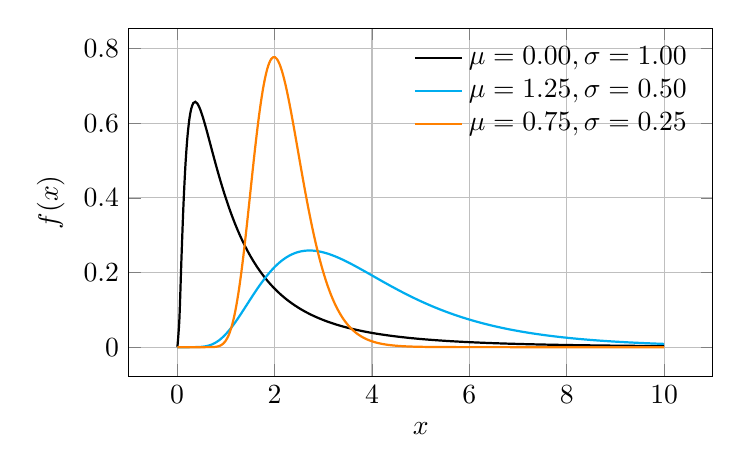
\begin{tikzpicture}[ declare function = { lognormal(\x,\mu,\sigma)=
        exp(-(ln(x)-\mu)^2/(2*\sigma^2))/(x*\sigma*(2*3.1415)^(0.5)); }]

      \def\parA{\mu} \def\parB{\sigma} \def\va{x}

  \begin{axis}[
    width = 9cm, height = 6cm,
    samples = 250, smooth, domain = -0.2:10,
    xlabel = $\va$, ylabel = $f(\va)$,
    grid=both,
%     xlabel style = {at = {(1,0)}, anchor = north west},
%     ylabel style = {rotate = -90, at = {(0,1)}, anchor = south east},
    legend style = {draw = none, fill = none}, clip = false]

    \only<+->{\addplot[black, thick] {lognormal(x, 0, 1)}; \addlegendentry{$\parA = 0.00, \parB = 1.00$};}

    \only<+->{\addplot[cyan, thick] {lognormal(x, 1.25, 0.5)}; \addlegendentry{$\parA = 1.25, \parB = 0.50$};}

    \only<+->{\addplot[orange, thick] {lognormal(x, 0.75, 0.25)}; \addlegendentry{$\parA = 0.75, \parB = 0.25$};}

    % \node[anchor = south] at (axis description cs: 0.5, 1.05)
    % {$f(\va) = \displaystyle\frac{1}{\va \parB \sqrt{2 \pi}}
    % \exp\left\{-\frac{\left(\ln(\va) - \parA\right)^2}{2 \parB^2}
    % \right\}$};
  \end{axis}
\end{tikzpicture}
\end{center}
  
\end{frame}

\begin{frame}
  \frametitle{Mean, median and variance of a lognormal distribution}\pause
  Let $X\sim \mathcal{LN}(\mu,\sigma^{2})$\pause
  
  \begin{block}{Mean}\pause
    The mean of $X$ is given by
    \pause
    
  \begin{equation}
    \label{eq:15}
    \mathbb{E}(X) = e^{\lt(\mu + \fr12 \sigma^2\rt)}
  \end{equation}
\end{block}


  \pause

  \begin{block}{Median}\pause
  The median of $X$ is:\pause

  \begin{equation}
    \label{eq:17}
    Median(X) = e^\mu
  \end{equation}
\end{block}

\begin{block}{Variance}\pause
  The variance of $X$ is given by:

  \pause
  
  \begin{equation}
    \label{eq:16}
    \mathbb{V}(X) = \pause   (e^{\sigma^2} - 1)e^{(2\mu + \sigma^{2})}
  \end{equation}
\end{block}
\end{frame}


\begin{frame}
  \frametitle{Example 1: Mean and variance  of   lognormal distribution (1)}
  \pause

  The incubation period of the COVID-19 infection is assumed to be lognormally distributed with a median of about 5
  days and $\sigma^{2} = 0.42$. What are the mean and variance of its distribution?
  \pause

  \begin{exampleblock}{Solution}\pause
    First, we find the parameter $\mu$: \pause
    \begin{eqnarray*}
      Median(X) &=& e^{\mu} \\\pause
      5 &=& e^{\mu} \\\pause
      \implies \ln(5) &=& \pause \mu \\\pause
      \therefore \text{The mean is given by } \pause \mathbb{E}(X) &=& e^{\mu + \fr12\sigma^{2}} \pause = e^{\ln(5) + 0.21}\\\pause
                &=& 5(e^{0.21}) \pause = \boxed{6.17 \text{ days}}
    \end{eqnarray*}
  \end{exampleblock}
\end{frame}

\begin{frame}
  \frametitle{Example 1: Mean and variance  of   lognormal distribution (2)}
  \pause

 
  \begin{exampleblock}{Solution (cont.)}\pause
    The variance is given by:\pause
    \begin{eqnarray*}
      \mathbb{V}(X) &=& \lt(\exp(\sigma^{2}) - 1 \rt)\lt(\exp[2\mu + \sigma^{2}]\rt) \\\pause
             &=& (\exp(0.42)-1)(\exp(2\ln(5) + 0.42)) \\\pause
             &=& \boxed{19.86 \text{ days}^{2}}
    \end{eqnarray*}
  \end{exampleblock}
\end{frame}

\begin{frame}
  \frametitle{Relationship between normal and lognormal distributions}\pause
  
  \begin{itemize}
  \item A random variable $\rd X$ is {\rd lognormally} distributed with the \textbf{parameters} $\mu$ and $\sigma^{2}$ if $\bl \ln(X)$
    is {\bl normally} distributed with the same parameters. \pause
    \begin{equation}
    {\rd  X \sim \mathcal{LN}(\mu,\sigma^{2}) } \pause \implies {\bl \ln(X) \sim \mathcal{N}(\mu,\sigma^{2})}
    \end{equation}
    \pause
    
  \item Conversely, a random variable $\bl X$ is {\bl normally} distributed with the parameters $\mu$ and $\sigma^{2}$ then
    $\rd e^{X}$ is {\rd lognormally} distributed with the same parameters.\pause
    \begin{equation}
     {\bl  X \sim \mathcal{N}(\mu,\sigma^{2})} \pause \implies \pause {\rd  e^{X} \sim \mathcal{LN}(\mu,\sigma^{2})}
    \end{equation}
    \pause
    
  \item If $X\sim \mathcal{N}(\mu, \sigma^{2})$, then $\mu = \mathbb{E}(X)$ and $\sigma^{2} = \mathbb{V}(X)$ \pause

    \bigskip
    
  \item However, $X\sim \mathcal{LN}(\mu, \sigma^{2})$, then $\mu = E(\ln(X))$ and $\sigma^{2} = \mathbb{V}(\ln(X))$\pause
    
  \end{itemize}

\end{frame}

\begin{frame}[shrink=25]
  \frametitle{Relationship between normal and lognormal (cont.)}\pause
  \tikzset{declare function={
    N(\x,\m,\SIG) = 1/(sqrt(2*pi))*exp(-0.5*(pow((\x-\m),2))/(2*\SIG^2));       
    L(\x,\m,\SIG) = 1/(\x*\SIG*sqrt(2*pi))*exp(-0.5*(pow((ln(\x)-\m),2))/(2*\SIG^2));}
}


     
    %\foreach \FZero in {0}
    %{
    \def\FZero{0}       %x coordinate on Normal distribution you want to project
    \def\Nmu{0.01}      %mu cannot b <= 0
    \def\Nsig{0.25}     %
    \pgfmathsetmacro{\Lmu}{ln(\Nmu)-0.5*\Nsig*\Nsig} 
    \pgfmathsetmacro{\Lsig}{ln(1+ \Nsig / \Nmu*\Nmu)}
    \pgfmathsetmacro{\Lb}{\Nmu-5*\Nsig}
    \pgfmathsetmacro{\Rb}{\Nmu+5*\Nsig}
    
    \pgfplotsset{
        Lnorm/.style={smooth,ultra thick,color=cyan!60!black,domain=\Lb:\Rb,samples=101},
        Llognorm/.style={color=cyan!60!black,ultra thick,domain=0.01:{exp(\Rb)},
        samples=201},
        Lexp/.style={color=green!50!black,ultra thick,domain=\Lb:\Rb,samples=101},
    }
    
    \begin{tikzpicture}
    \begin{groupplot}[
        group style={group size=2 by 2,
                     horizontal sep=0pt,
                     vertical sep=0pt,
                     xticklabels at=edge bottom,
                     yticklabels at=edge left
                     },
                     % customaxis2,                   
                     height=8cm,
                     width=8cm,
                     legend pos=north east,grid=major,
    %                grid=both
                     ]
    % top left
%    \only<1->{
     \nextgroupplot[group/empty plot]
   %                }
    % top right
    %\only<4->{    
    \nextgroupplot[ymax=1.8,xmin=0]
        \addplot[name path=TR1,Llognorm]                {L(x,\Nmu,\Nsig)} ;
        \addplot[name path=TR2,Llognorm,opacity=0.5]    {L(x,{\Nmu +0.3},\Nsig)} ;
        \addplot[name path=TR3,Llognorm,opacity=0.25]   {L(x,{\Nmu +0.5},\Nsig)} ;
        \addlegendentry{$X \sim \mathcal{LN}(0,\Nsig^{2})$}
        \node[circle,draw, green, thick] (c1) at (axis cs:{exp(\FZero)},{L({exp(\FZero)},\Nmu,\Nsig)}) {};
        \node at (3.7,0) {$x$};
     %  }
        % bottom left
    %\only<2->{
    \nextgroupplot[xmin=-0,y coord trafo/.code={\pgfmathparse{-####1}},
                    y coord inv trafo/.code={\pgfmathparse{-####1}}]
        \addplot[name path=BL1,Lnorm]               ({N(x,\Nmu,\Nsig)},{x}) ;
        \addplot[name path=BL2,Lnorm,opacity=0.5]   ({N(x,{\Nmu+0.5},\Nsig)},{x}) ;
        \addplot[name path=BL3,Lnorm,opacity=0.25]  ({N(x,{\Nmu+1},\Nsig)},{x}) ;
        \addlegendentry{$Y \sim \mathcal{N}(0,\Nsig^{2})$}
        \node[circle,draw,green,thick] (a1) at (axis cs:{N(\FZero,\Nmu,\Nsig)},\FZero) {};
        \node at (0.01,-1.3) {$y$};
     % }
     %bottom right
        \nextgroupplot[%yticklabels={},
        xmin=0,
                    y coord trafo/.code={\pgfmathparse{-####1}},
                    y coord inv trafo/.code={\pgfmathparse{-####1}}]
        \addplot[name path=BR1,Lexp] ({exp(x)},{x}) node[right,pos=0.5] {$x=e^{y}$};
        \addlegendentry{$x=e^y$}
        \node[circle,draw, green, thick] (b1) at (axis cs:{exp(\FZero)},\FZero) {};
    \end{groupplot}
  
  
    %Connect points between groupplots
    \draw[-latex,dashed,green!50!black,thick] (a1) -- (b1) -- (c1) ;
    
    \end{tikzpicture}
    %}
\end{frame}


\begin{frame}
  \frametitle{Positive skewness of lognormal distribution}
  \pause

  \begin{itemize}[<+->]
  \item The lognormal distribution is positively skewed
  \item Its mean is always greater than its median
  \end{itemize}

  \pause

  \bigskip
  
    \begin{center}
    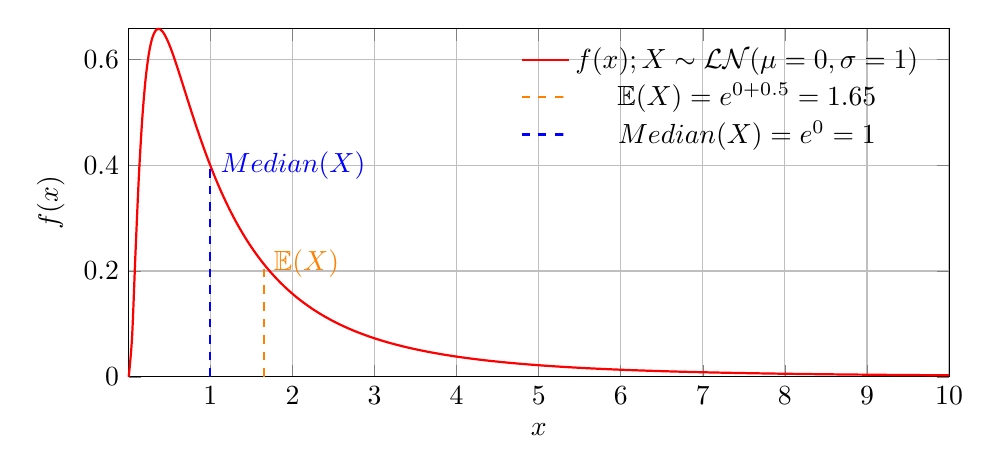
\begin{tikzpicture}[ declare function = { lognormal(\x,\mu,\sigma)=
        exp(-(ln(x)-\mu)^2/(2*\sigma^2))/(x*\sigma*(2*3.1415)^(0.5)); }]

      \def\parA{\mu} \def\parB{\sigma} \def\va{x}

  \begin{axis}[
    width = 12cm, height = 6cm,
    samples = 250, smooth, domain = -0.2:10,
    xlabel = $\va$, ylabel = $f(\va)$,
    grid=both,
%     xlabel style = {at = {(1,0)}, anchor = north west},
%     ylabel style = {rotate = -90, at = {(0,1)}, anchor = south east},
    legend style = {draw = none, fill = none}, clip = false, enlargelimits=false]

    \addplot[red, thick] {lognormal(x, 0, 1)};
    \addlegendentry{$f(x); X \sim \mathcal{LN}(\parA = 0, \parB = 1)$};
    \addplot[orange, thick, dashed] coordinates {(1.649,0) (1.649, {lognormal(1.649,0,1)})} node[right] {$\mathbb{E}(X)$};
    \addlegendentry{$\mathbb{E}(X) = e^{0 + 0.5}= 1.65 $};
    \addplot[blue, thick, dashed] coordinates {(1,0) (1, {lognormal(1,0,1)})} node[right] {$Median(X)$};
    \addlegendentry{$Median(X) = e^{0}=1$}; %, \mathbb{V}(X) = (e-1)e$};
    % \addplot[cyan, thick] {lognormal(x, 1.25, 0.5)}; \addlegendentry{$\parA = 1.25, \parB = 0.50$};

    % \addplot[orange, thick] {lognormal(x, 0.75, 0.25)}; \addlegendentry{$\parA = 0.75, \parB = 0.25$};

    % \node[anchor = south] at (axis description cs: 0.5, 1.05)
    % {$f(\va) = \displaystyle\frac{1}{\va \parB \sqrt{2 \pi}}
    % \exp\left\{-\frac{\left(\ln(\va) - \parA\right)^2}{2 \parB^2}
    % \right\}$};
  \end{axis}
\end{tikzpicture}
\end{center}
\end{frame}


% \begin{frame}
%   \frametitle{Lognormal distribution (cont.)}

%   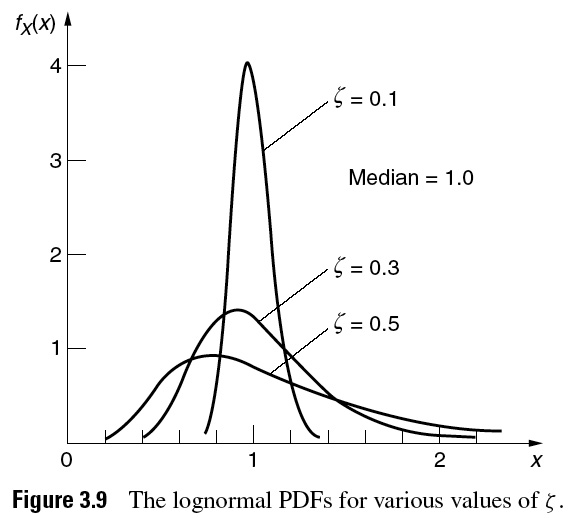
\includegraphics[width=.8\textwidth]{03_09}
% \end{frame}

\begin{frame}
  \frametitle{Probability of a lognormal random variate}
    Given a r.v.\ $X$ that is lognormally distributed with parameters $\mu$ and $\sigma^2$:

  \begin{equation}
    \label{eq:12}
    P(a < X \le b) = \pause \fr{1}{\sigma x\sqrt{2\pi}} \pause \int_a^b e^{-\fr12\lt(\fr{\ln(x)-\mu}{\sigma}\rt)^2}dx
  \end{equation}

  \pause

  \bigskip
  
  Substituting $z = \fr{\ln(x)-\mu}{\sigma}\pause \implies\pause dx = \sigma xdz$, we obtain: \pause

  \begin{equation}
     P(a < X \le b) \pause = \fr{1}{\sqrt{2\pi}}\int_{(\ln(a)-\mu)/\sigma}^{(\ln(b)-\mu)/\sigma} \pause e^{-\fr12z^2}dz    
  \end{equation}
  \medskip
  
  \pause

  Recognizing that the integrand is the PDF of the \textbf{\rd standard normal distribution}, we have: \pause

  \begin{equation}
    \rd
    P(a < X \le b) \pause  =  \Phi\lt(\fr{\ln b-\mu}{\sigma}\rt) \pause -\pause  \Phi\lt(\fr{\ln a-\mu}{\sigma}\rt)
  \end{equation}
\end{frame}

% \begin{frame}
%   \frametitle{Further relationships between lognormal parameters}\pause
  
%   Refer to pages 102-103 in your text for these derivations. \pause
%   \begin{align}
%     \zeta^2 &= \ln(1 + \delta_X^2) \\ \pause
%     \implies \zeta &\approx \delta_X
%   \end{align}

%   \begin{align}
%     \mu_X &= x_m\sqrt{1 + \delta_X^2} \\ \pause
%     \implies \mu_X & > x_m
%   \end{align}
% \end{frame}


\begin{frame}
  \frametitle{Example 2: Equipment breakdown}\pause
  The lifetime $X$ of a major oil platform equipment is lognormally distributed with a
  $Median(X) =6$ months and $\sigma = 0.30$.  To ensure 95\% reliability, determine the desired interval $x_{0}$ for
  maintenance.\\ \pause

    \bigskip
    
    \begin{exampleblock}{Solution}\pause
      Given: $\mu = \ln 6 = 1.792$ and $\sigma = 0.30$, we want to find $x_0$ such that: \pause
      \begin{equation*}
        P(X > x_0) = 1 - P(X\le x_0) = \pause 0.95
      \end{equation*}
      \pause

      Thus:
      \begin{equation*}
        \Phi\lt(\fr{\ln(x_0) - 1.792}{0.30}\rt) = \pause 0.05
      \end{equation*}
    \end{exampleblock}
 \end{frame}


\begin{frame}
  \frametitle{Example 2: Equipment breakdown (cont.)}
    \pause

       \begin{exampleblock}{Solution}\pause
        \begin{eqnarray*}
          \fr{\ln x_0 - 1.792}{0.30} &=& \Phi^{-1}(0.05) \\ \pause
          \ln x_0 - 1.792 &=&  \pause 0.30[- \Phi^{-1}(0.95)] \\ \pause
          \ln x_0       &=& 1.792 +  0.30(-1.65) \\\pause
                                     &=& 1.792 -0.495 = \pause 1.297
        \end{eqnarray*}
        \pause

        Therefore, the required inspection interval is:
        \begin{equation*}
          x_0 = \pause  e^{1.297} = \pause 3.66 \text{ months}
        \end{equation*}
      \end{exampleblock}

 \end{frame}

\section{Exponential distribution}
\begin{frame}
  \frametitle{Modeling probabilities of elapsed times}
  \pause
  Consider the random variable $\rd X$ which represents the \textit{\rd number of arrivals} at a restaurant within a given time interval.
  \pause

  \begin{center}
    
\includegraphics[width=.7\textwidth,trim={0 3cm 0 0.5cm},clip]{cafe}
  \end{center}
  \pause
  
  \begin{itemize}
    % \item $X$ represents a Poisson process \pause
  \item The probability of $X$ in $t$ time units can be modeled by the Poisson distribution with a rate parameter $\la t$
  \end{itemize}

   
  \pause

  \begin{exampleblock}{}
    Now consider the variable $\gr Y$ representing the \textbf{\gr elapsed time} between successive arrivals. \pause

    \begin{itemize}
    \item What is the probability the time between the third and fourth arrivals is less than $y$ minutes, for instance?\pause
    \item This is modeled by the \textbf{\gr exponential distribution} with parameter $\la$.
    \end{itemize}
  \end{exampleblock}

\end{frame}
\begin{frame}
  \frametitle{Exponential distribution}
  \pause

  \begin{block}{Definition}\pause
    A random variable $X$ that is exponentially distributed with parameter $\la$ has the PDF:\pause
    \begin{equation}
      f_{X}(x) = \pause \la e^{-\la x} \pause \qquad x > 0
    \end{equation}
  \end{block}
  \pause

  \begin{center}
      \begin{tikzpicture}
      \begin{axis}[no marks, width=10cm, height=5cm,
        samples = 100,
        axis x line=center,
        axis y line=center,
        xtick={0,1,2,...,8},
        ytick={0,0.25,...,2},
        domain = 0:8,
        xlabel={$t$},
        ylabel={$f_T(t)$},
        xlabel style={right},
        ylabel style={above },
        ymax=2.1,
        xmax=8.2,
        %x post scale=1.7,
        enlargelimits=false,
        grid=both,
        yticklabel style={
          /pgf/number format/fixed,
          /pgf/number format/fixed zerofill,
          /pgf/number format/precision=2
        }
        ]
        \addplot+[draw=orange,   thick,opacity=1] {expo(.5,x)}; \addlegendentry{ $\la = 0.5$}
        \addplot+[draw=red,   thick,opacity=1] {expo(1,x)}; \addlegendentry{ $\la = 1.0$}
        \addplot+[draw=green!50!black,   thick,opacity=1] {expo(1.5,x)}; \addlegendentry{ $\la = 1.5$}
        \addplot+[draw=blue,   thick,opacity=1] {expo(2,x)}; \addlegendentry{ $\la = 2.0$}        
%        \addplot+[draw=black,thick, pattern=north east lines, opacity=1, domain=0:1] {expo(1.5,x)} \closedcycle; 
      \end{axis}
    \end{tikzpicture}
\end{center}
  
\end{frame}

\begin{frame}
  \frametitle{CDF of the exponential distribution}
  \pause
  The CDF of the exponential distribution is derived as:\pause
  \begin{eqnarray*}
    F_{X}(x) &=& \pause P(X\le x)\pause = \int_{0}^{x}\la e^{-\la t}dt \\\pause
    F_{X}(x)         &=& 1 - e^{-\la x} 
  \end{eqnarray*}
  \pause
    \begin{center}
      \begin{tikzpicture}
      \begin{axis}[no marks, width=10cm, height=5cm,
        samples = 100,
        axis x line=center,
        axis y line=center,
        xtick={0,1,2,...,8},
        ytick={0,0.25,...,2},
        domain = 0:8,
        xlabel={$t$},
        ylabel={$F_T(t)$},
        xlabel style={right},
        ylabel style={above },
        ymax=1.1,
        xmax=8.2,
        %x post scale=1.7,
        enlargelimits=false,legend style={at={(1,.5)},anchor= east},
        grid=both,
        yticklabel style={
          /pgf/number format/fixed,
          /pgf/number format/fixed zerofill,
          /pgf/number format/precision=2
        }
        ]
        \addplot+[draw=orange,   thick,opacity=1] {expocdf(.5,x)}; \addlegendentry{ $\la = 0.5$}
        \addplot+[draw=red,   thick,opacity=1] {expocdf(1,x)}; \addlegendentry{ $\la = 1.0$}
        \addplot+[draw=green!50!black,   thick,opacity=1] {expocdf(1.5,x)}; \addlegendentry{ $\la = 1.5$}
        \addplot+[draw=blue,   thick,opacity=1] {expocdf(2,x)}; \addlegendentry{ $\la = 2.0$}        
%        \addplot+[draw=black,thick, pattern=north east lines, opacity=1, domain=0:1] {expo(1.5,x)} \closedcycle; 
      \end{axis}
    \end{tikzpicture}
\end{center}
\pause

Note that $\bl P(X\le x) = 1 - e^{-\la x}$, \pause while $\rd P(X > x) = 1 - (1 - e^{-\la x}) = e^{-\la x}$
\end{frame}

\begin{frame}
  \frametitle{Mean and variance of the exponential distribution}
  \pause
  Let $X \sim \text{Exponential}(\la)$.\pause
  
  \begin{block}{Mean}
    The mean of $X$ is given by: \pause
    \begin{equation}
      \mathbb{E}(X) \pause = \fr{1}{\la}
    \end{equation}
  \end{block}

  \pause

  \begin{block}{Variance}
    The variance of $X$ is given by: \pause
    \begin{equation}
      \mathbb{V}(X) \pause = \pause \fr{1}{\la^{2}}
    \end{equation}
  \end{block}
\end{frame}

\begin{frame}
  \frametitle{Example 3: Waiting for a flight}
  \pause
  The delay time  $T$ of a flight is exponentially distributed wtih $\la = 2$ (delays per hour). \pause Answer the following questions:
  \begin{enumerate}[\bf (a)]
  \item What is the mean delay (waiting) time, $\mathbb{E}(T)$?
  \item What is the variance of the delay time $\mathbb{V}(T)$?
  \item Find the probability that a flight will be delayed by no more than 10 minutes.
  \item Assuming you have been waiting for a flight for an hour, what is the probability that the flight will be delayed
    for an additional 30 minutes? (i.e.\ Find $P(T>1.5|T>1)$).
  \end{enumerate}
  
\end{frame}

\begin{frame}
  \frametitle{Example 3: Waiting for a flight (cont.)}
  \pause

  \begin{exampleblock}{Solution}
    \begin{enumerate}[\bf (a)]\setcounter{enumi}{0}
    \item The mean delay is given by \pause
      \begin{eqnarray*}
        E(T) &=&\pause \fr{1}{\la} \pause = \fr{1}{2} \pause =  \boxed{\gr 0.5 \text{hr}}
      \end{eqnarray*}
      \pause

    \item The variance is: \pause
      \begin{eqnarray*}
        \mathbb{V}(T) &=& \fr{1}{\la^{2}} \pause = \fr{1}{2^{2}} = \pause \boxed{\gr 0.25 \text{hr}^{2}}
      \end{eqnarray*}
    \end{enumerate}
  \end{exampleblock}
\end{frame}

\begin{frame}
  \frametitle{Example 3: Waiting for a flight (cont.)}
  \pause

  \begin{exampleblock}{Solution}
    \begin{enumerate}[\bf (a)]\setcounter{enumi}{2}
    \item The probability the flight will be delayed by no more than 10 minutes ( $\fr16$ hr) is given by: \pause
      \begin{eqnarray*}
        P\lt(T \le \fr16\rt) &=& 1 - e^{-\la \cdot\fr16} \pause = 1 - e^{-2\lt(\fr16\rt)} \\\pause
                       &=& 1 - e^{-\fr13} \pause = \boxed{0.283}
      \end{eqnarray*}
    \end{enumerate}
  \end{exampleblock}
\end{frame}

\begin{frame}
  \frametitle{Example 3: Waiting for a flight (cont.)}
  \pause

  \begin{exampleblock}{Solution}
    \begin{enumerate}[\bf (a)]\setcounter{enumi}{3}
    \item The probability that the flight will be delayed by a further 0.5hr after 1hr of waiting is given by:\pause
      \begin{eqnarray*}
        P(T > ( 0.5 + 1) | T > 1) &=& P(T > 1.5 |T > 1) \\\pause
                                    &=& \fr{P((T > 1.5) \cap  (T > 1))}{P(T > 1)} \pause \quad \text{\og (mult.\
                                        rule)} \\ \pause
                                  &=& \fr{P(T > 1.5)}{P(T > 1)} \\ \pause
                                  &=& \fr{e^{-2(1.5)}}{e^{-2(1)}} \pause = e^{-2[1.5 - 1.0]} \\\pause
                                  &=& e^{-2(0.5)} \quad (=P(T > 0.5)) \\\pause
                                  &=& e^{-1} \pause = \boxed{\gr 0.37}
      \end{eqnarray*}
    \end{enumerate}
  \end{exampleblock}
\end{frame}

\begin{frame}
  \frametitle{Memorylessness of the exponential distribution}
  \pause
  This leads us to an important property of the exponential distribution
  \pause

  \begin{block}{Memoryless property}
    \begin{equation}
    P(T > t + s | T > s) = \pause P(T > t)
  \end{equation}
  \pause

  That is, it does not matter from which time the waiting begins (i.e.\ conditioning); the probability of an elapsed time remains the same.
  \end{block}
\end{frame}

\section{Outlook}
\begin{frame}
  \frametitle{Recap}
  \begin{itemize}
  \item \textbf{Lognormal distribution:} $X\sim \mathcal{LN}(\mu,\sigma^{2})$\\
    CDF: $F_{X}(x) = P(X\le x) = \Phi((\ln(x) - \mu)/\sigma)$\\\pause
    \pause
    Mean:
    \begin{equation}
      \label{eq:15}
      \mathbb{E}(X) = e^{\lt(\mu + \fr12 \sigma^2\rt)}
    \end{equation}
    \pause    
    Variance:
      \begin{equation}
    \label{eq:16}
    \mathbb{V}(X) = \pause   (e^{\sigma^2} - 1)e^{(2\mu + \sigma^{2})}
  \end{equation}
    
  \item \textbf{Exponential distribution}: $X \sim \text{Exponential}(\la)$
    \pause
    \begin{eqnarray}
      \text{PDF:}\quad  f_{X}(x) &=& \pause \la e^{-\la x}, \pause \qquad x > 0 \\
      \text{CDF:}\quad  F_{X}(x) &=& P(X \le x) = \pause  1 - e^{-\la x}, \pause \qquad x > 0 
    \end{eqnarray}

    \pause

    Mean:
    \begin{equation}
      \mathbb{E}(X) = \fr{1}{\la}
    \end{equation}

    \pause

    Variance:
    \begin{equation}
      \mathbb{V}(X) = \fr{1}{\la^{2}}
    \end{equation}
  \end{itemize}
\end{frame}

\begin{frame}
  \frametitle{MATLAB Homework}
  \pause

  \begin{itemize}
  \item Ensure your submission is strictly a script saved with the \texttt{\rd .m} extension
    \pause
    \medskip
    
  % \item Subsequent templates will include \texttt{clc} and \texttt{clear all} at the beginning of the script to facilitate grading by the TA
  %   \pause
  %   \medskip
    
  \item MATLAB can only execute a script if it is in the \textit{\rd current folder}. \pause Otherwise you may get a message like the one below:
    \pause 
    \begin{center}
      
\includegraphics[width=.4\textwidth]{matlab}
    \end{center}
    \pause
    If so, simply click on \texttt{Change Folder} or move the file to the current folder you are in. Finally, always make sure the path of a file being read by a script is valid from its location, otherwise you will have to deal with ``File not found'' errors.
  \end{itemize}
\end{frame}


\begin{frame}
  \frametitle{Midterm Exam}
  \pause

  \begin{itemize}
  \item 24-hour open-resource examination
    \pause

    \medskip
    
  \item Available for download via Canvas on Wednesday, October 16th at \textbf{10:00 AM}\pause
    \medskip

  \item Due by \textbf{October 21st} at \textbf{11:59 PM}\pause
    \medskip

  \item Exam length will be similar to previous midterms or the practice exam(s) available on Canvas.
    \pause
    \medskip
    
  \item Exam is designed to be completed in 2-3 hours or less. \pause The 24-hr window gives you flexibility and time to
    plan, organize and check your work before submission.
    \pause
    \medskip

  \item You can use your calculator/computer (Matlab/Python) to compute probabilities (as long as you indicate how you obtained your answer).

%  \item \bl Next lecture (Tuesday, October 6th) will be a \textbf{Midterm Review Session}
  \end{itemize}
\end{frame}

% \section{Joint distributions}

% \begin{frame}
%   \frametitle{Joint distributions}\pause
%   Given two random variables $X$ and $Y$:

%   \begin{block}{Discrete case}
%     The joint PMF is:
%     \begin{equation}
%       \label{eq:62}
%       p_{X,Y}(x_i,y_j) = P(X=x_i, Y = y_j)
%     \end{equation} \pause
%     The CDF is:
%     \begin{equation}
%       \label{eq:63}
%       F_{X,Y}(x,y) = \sum_{x_i \le x}\sum_{y_j \le y} p_{X,Y}(x_i, y_j)
%     \end{equation}
%   \end{block}
%   \pause

%   \begin{block}{Continuous case}\pause
%     The joint probability is given by:
%     \begin{equation}
%       P(a < X \le b, c < Y \le d) = \int_a^b \int_c^d f_{X,Y}(x,y)dy dx
%     \end{equation}
%   \end{block}
% \end{frame}

% \begin{frame}
%   \frametitle{Joint and marginal distributions} \pause

%   Marginal distributions: $P(x_1)$, $P(x_2)$ \\ \pause
%   Joint distribution: $P(x_1,x_2)$. \pause
  
%   \pgfplotsset{
%     colormap={whitered}{color(0cm)=(white); color(1cm)=(purple!75!blue)}
%   }

%   \begin{tikzpicture}[scale=.6,
%     declare function={mu1=1;},
%     declare function={mu2=2;},
%     declare function={sigma1=0.5;},
%     declare function={sigma2=1;},
%     declare function={normal(\m,\s)=1/(2*\s*sqrt(pi))*exp(-(x-\m)^2/(2*\s^2));},
%     declare function={bivar(\ma,\sa,\mb,\sb)=
%       1/(2*pi*\sa*\sb) * exp(-((x-\ma)^2/\sa^2 + (y-\mb)^2/\sb^2))/2;}]
%     \begin{axis}[
%       colormap name=whitered,
%       width=15cm,
%       view={45}{65},
%       enlargelimits=false,
%       grid=major,
%       domain=-1:4,
%       y domain=-1:4,
%       samples=26,
%       xlabel=$x_1$,
%       ylabel=$x_2$,
%       zlabel={$P$},
%       colorbar,
%       colorbar style={
%         at={(1.1,0)},
%         anchor=south west,
%         height=0.25*\pgfkeysvalueof{/pgfplots/parent axis height},
%         title={$P(x_1,x_2)$}
%       }
%       ]
%       \only<4->{\addplot3 [surf] {bivar(mu1,sigma1,mu2,sigma2)};}
%       \only<5->{\addplot3 [domain=-1:4,samples=31, samples y=0, red, thick, smooth] (x,4,{normal(mu1,sigma1)});}
%       \only<6->{\addplot3 [domain=-1:4,samples=31, samples y=0, blue, thick, smooth] (-1,x,{normal(mu2,sigma2)});}

%       \only<7->{\draw [black!50] (axis cs:-1,0,0) -- (axis cs:4,0,0);}
%       \only<8->{\draw [black!50] (axis cs:0,-1,0) -- (axis cs:0,4,0);}

%       \only<9->{\node[blue] at (axis cs:-1,1,0.18) [pin=165:$P(x_1)$] {};}
%       \only<10->{\node[red] at (axis cs:1.5,4,0.32) [pin=-15:$P(x_2)$] {};}
%     \end{axis}
%   \end{tikzpicture}
% \end{frame}

%\begin{frame}[allowframebreaks]
%   \frametitle{References}
%   \AtNextBibliography{\scriptsize}
%   \setbeamertemplate{bibliography item}[text]
%   \printbibliography[heading=none]
  
% \end{frame}

%\printbibliography
\end{document}
%%% Local Variables:
%%% mode: latex
%%% TeX-master: t
%%% End:
